\documentclass[12pt]{article}

% TEMPLATE DEFAULT PACKAGES
\usepackage{amssymb,amsmath,amsfonts,eurosym,geometry,ulem,graphicx,caption,color,setspace,sectsty,comment,footmisc,caption,natbib,pdflscape,subfigure,array,hyperref}

% ADDED PACKAGES FOR THIS MANUSCRIPT
\usepackage{mathptmx,multirow,titlesec,threeparttable,tabu,booktabs}
% endfloat,

% SECTION TITLE SETTINGS
\titlelabel{\thetitle.\enskip}
\titleformat*{\section}{\large\bfseries}
\titleformat*{\subsection}{\normalsize\bfseries}

% COLUMN TYPES
\newcolumntype{L}[1]{>{\raggedright\let\newline\\\arraybackslash\hspace{0pt}}m{#1}}
\newcolumntype{C}[1]{>{\centering\let\newline\\\arraybackslash\hspace{0pt}}m{#1}}
\newcolumntype{R}[1]{>{\raggedleft\let\newline\\\arraybackslash\hspace{0pt}}m{#1}}

% MARGINS AND SPACING
\normalem
%\onehalfspacing
\geometry{left=1.0in,right=1.0in,top=1.0in,bottom=1.0in}

% SPECIAL CELL 
\newcommand{\specialcell}[2][c]{%
	\begin{tabular}[#1]{@{}l@{}}#2\end{tabular}}

\begin{document}

\begin{titlepage}
\title{In da house!\thanks{I am grateful to Matthew Turner and Jesse Shapiro for their feedback, advice and support. I also thank Nathaniel Baum-Snow, John Friedman, Nicolas Gendron-Carrier, William Violette, Jacob Robbins, and all the participants of the Brown University applied microeconomics seminar for their helpful comments. I am indebted to Aaron Kilbey for granting me access to a beta version of Portland Maps's API and allowing me to complete the data collection for this project. Ian Hackett also provided invaluable help in obtaining data necessary for this project. Finally, financial support from the Fonds de Recherche Soci\'et\'e et Culture du Qu\'ebec is gratefully acknowledged.}}
\vspace{2mm}
\author{Stefano Polloni\thanks{Department of Economics, Brown University, Box B, Providence, RI 02912  E-mail: stefano\textunderscore polloni@brown.edu}\\[-0.4em] \normalsize{\it Brown University}\\}
\vspace{30mm}
\date{\vspace{5mm}This Version: \today}
\maketitle
\begin{abstract}
\noindent We estimate economic spillovers from subsidized housing projects on local neighborhoods using housing transaction records and high-resolution census data in South Africa.  With a differences-in-differences design, we find that projects lead to a X\% decline in nearby housing prices.  We attribute this decline to externalities from informal settlements constructed within housing projects.   \\
\vspace{0in}\\
\noindent\textbf{Keywords:} traffic externalities; street livability; urban policy; housing market.\\
\vspace{0in}\\
\noindent\textbf{JEL Codes:} O18; H4; R2; R4.\\

\bigskip
\end{abstract}
\setcounter{page}{0}
\thispagestyle{empty}
\end{titlepage}
\pagebreak \newpage

\doublespacing

\section{Introduction} \label{sec:introduction}


In developing countries, 30\% of urban populations live in slums where households often suffer high rates of crime, low access to infrastructure, insecure property rights, and unsanitary conditions (\cite{mdg}).  These negative externalities often combine to create poverty traps, preventing long-term economic development (\cite{10.1257/jep.27.4.187}). Governments have responded by replacing slums with new homes and moving slum dwellers to public housing projects.  While these policies are often motivated by immediate health and economic benefits for recipients, economic theory emphasizes how high-quality public housing provides an incentive for neighbors to invest more in their own homes and communities, reducing negative externalities and steering communities away from poverty traps.

In this paper, we analyze the impacts of public housing on the development of surrounding neighborhoods.  We study a large-scale housing program in South Africa, which has allocated over 4.3 million dwellings and houses over 13\% of the total population (\cite{dhsreports}; GHS 2009-2013).  Already one of the largest housing programs in the developing world, this program continues to respond to large backlogs in housing demand with an even mix of upgrading slum areas with new houses as well as constructing large public housing developments.  This program is intended to not only serve as ``a key strategy for poverty alleviation'' for direct beneficiaries, but also generate community-wide benefits, ``leveraging growth in the economy,'' ``combating crime, promoting social cohesion and improving quality of life for the poor,'' and ``utilizing housing as an instrument for the development of sustainable human settlements, in support of spatial restructuring'' (\cite{bng}). 

We combine administrative data on [XX] housing projects with data on property transactions, demographics, and building construction to measure the local impacts of these projects.  We estimate a persistent [XX]\% decline in home prices within [XX] meters of a project.  We then use heterogeneity in the extent to which projects eradicate existing slums as a natural experiment to quantify negative externalities from slum areas.  Our estimates imply that increasing slum density by [XX]\% leads to a [XX]\% decline in local housing prices.  We find some evidence that this effect scales non-linearly with the size of the housing projects, which has theoretical implications for the extent to which slum areas represent poverty traps.

To identify these effects, we use a differences-in-differences strategy leveraging both the exact timing of housing project construction as well as precise geographic proximity of surrounding areas.  Like \cite{diamond2016wants}'s similar analysis of public housing in the US, we leverage the substantial uncertainty in project timing due to difficulties coordinating many stakeholders and sources of funding (\cite{serihistory}).  Similar to the context in the US, we find little evidence that local housing markets anticipate these projects.  We also build on \cite{diamond2016wants} by using planned but unconstructed project areas as counterfactual areas, which help to control for demographic or housing market trends that might be correlated with the choice of project locations.

Our negative spillover estimates stand in contrast to a large literature in development that has focused on measuring housing impacts on direct recipients.  Relying on small-scale experimental designs, previous studies have linked public housing to improvements in employment outcomes (\cite{franklin2016enabled}), self-reported wellbeing (\cite{galiani2017shelter}; \cite{devoto2012happiness}), and child health outcomes (\cite{cattaneo2009housing}).  Data limitations both in finding a large enough sample of housing projects and in identifying outcomes at a precise spatial scale have prevented previous studies identifying spillover effects.  Taken alongside these previous studies, our findings suggest that policymakers may benefit from weighing direct benefits to recipients against potential negative effects to the local housing neighborhoods in designing future housing policy.

To understand the welfare implications of this policy, we also develop a model similar to... 

%% COULD ALSO REFRAME ALL THIS TOP STUFF TO HAVE MORE WELFARE AND THEORY INVOLVED


\subsection{Where are houses built?}

Between 2000 and 2010, subsidized housing efforts in South Africa have primarily focused on constructing and allocating single-story, two-room (30 to 40 square meter) dwellings to households in groups of 50 to 500 per project.  These housing projects are evenly divided between two categories (\cite{dhsreports}):
\begin{enumerate}
	\item  \textbf{Greenfield developments} involve the construction of housing projects primarily on undeveloped state-owned land although in some cases, municipalities will work with private developers to purchase inexpensive, undeveloped private land for these projects.  Finding undeveloped land often requires policymakers to locate these projects far from city centers and economic opportunities.  
	\item  \textbf{In-situ upgradings} replace existing informal settlements with housing developments.\footnote{While in some cases these programs refer simply to the provision of land titles and municipal services (water, electricity, etc.), this paper focuses on cases where informal settlements are replaced by fully-serviced, single-story houses.}  Since informal settlements are often located closer to city centers, the resulting housing projects may provide better employment opportunities (\cite{serihistory}).
\end{enumerate}
Facing substantial housing demand, the Department of Human Settlements has continued to issue grants to provincial governments to keep the rate of yearly housing allocations roughly constant (\cite{dhsreports}).  While the location and types of projects are determined by provincial and municipal governments, construction is subcontracted to private developers who also act as project managers assisting in the allocation of houses to beneficiaries (\cite{seriq}).

Since housing projects require coordination between many stakeholders, these projects often face unanticipated delays and cancellations due to labor and land procurement issues, difficulties gaining support from local government agencies, environmental impact assessments, and inadequate bulk infrastructure provision (\cite{dhsreports}).  In one example, political disagreements with local stakeholders led to the abandonment of a large project in Gauteng (\cite{protest}).

\subsection{Who are the beneficiaries?}

The National Department of Human Settlements issues guidelines for eligibility and maintains an official waiting list for eligible households for greenfield developments.  Eligibility requires citizenship, no previous property ownership, being married or having financial dependents, and having a monthly household income below R3,500 (\cite{seriq}).\footnote{The Gauteng Province has implemented their own waiting list since 2008 in order to exert greater control over the allocation process.}  The share of households reporting at least one member on the waiting list has remained stable at over 13\% from 2009 to 2013.\footnote{This figure is calculated from the General Household Surveys from 2009 to 2013}  Before construction, each project is assigned beneficiaries in a first-come, first-served basis according to the waiting list in their province or municipality.  For in-situ upgrading projects, previous inhabitants of informal settlements receive renovated houses while any remaining houses are allocated according to the housing waiting list.

In practice, these guidelines are only loosely followed.  Recent reports point to cases of corruption in the allocation of houses while in some instances, housing projects are organized with the assistance of local community groups who ultimately select the beneficiaries (\cite{seriq}; \cite{casestudytinazonke}).  Research suggests that Beneficiaries are often selected over the course of project construction and sometimes even after construction has finished (\cite{seriq}).

Beneficiaries are expected to pay a small one-time payment in order to receive title for their houses.  Guidelines also prevent beneficiaries from reselling their houses (and discourage renting) within their first 7 years of ownership.  Despite these guidelines, only 82\% of project houses are reported being still occupied by their original beneficiaries within five years of construction.\footnote{This figure is calculated from the General Household Surveys from 2009 to 2013}  Anecdotal evidence suggests that project managers are aware of this active secondary market but have difficulty policing these transactions (\cite{resale}).

\section{Data}

Understanding the spillover impacts of public housing requires (1) outcome measures at high spatial and geographic resolutions as well as (2) a precise measure of the location, timing, and size of housing projects.  

\subsection{Measuring Spillover Outcomes}

To measure formal housing market impacts, we use over 500,000 housing transactions from the South African National Deeds Office covering the universe of transactions for suburbs in the bottom 20\% of the housing market between 2003 and 2011 in the Gauteng Province (including the Johannesburg metro area).\footnote{The bottom 20\% suburbs were selected relative to prices in 2003 and followed every year from 2003 to 2011.  These data were provided by the Affordable Land and Housing Data Centre, which tracks affordable housing markets.}  These data include the price, exact location, plot size, buyer name, and seller name for each transaction.  To isolate spillover effects, we focus on transactions occurring within 1.2 kilometers of a housing project bringing the final sample to around 100,000 transactions.  We exclude the top 1\% of prices as well as prices below 1,000 Rand, which are likely composed of measurement error or the exchange of property title between family members.

Since government deeds records are unlikely to capture informal housing markets, we also include a building census of all structures in the Gauteng Province in 2001 and 2011.  Using a combination of high-resolution satellite imagery and local field teams, these data record the precise location of each structure, identifying structures within over 30 categories including formal and informal residential dwellings.  Out of 3,817,840structures, this building census includes 1,628,073formal structures and 1,560,345informal structures.  This data serves as both an outcome measure of informal housing development as well as an additional measure for public housing construction.

For demographic and economic outcomes, we turn to the census of population for 2001 and 2011 as well as the yearly General Household Survey for 2005 through 2014.  Both surveys include information about dwelling type, employment, income, and demographics for each household.  The General Household Survey includes additional details on participation in housing programs over time for a random sample of around 35,000 households in the Gauteng Province.  To spatially link these households in both samples to their corresponding housing projects, we conduct the analysis at the census block level, which is the smallest geography available with 28,437blocks in the Gauteng Province and 20,457within 1.2 kilometers of a housing project.  

\subsection{Defining Housing Projects}

Our primary measure of housing projects matches a set of housing program characteristics using the transaction records in the deeds data.  This procedure results in clusters of dwellings that form our housing projects (\cite{serihistory}).



\subsubsection{Seller Identity:}
% prob yes and large : 2770 / 127600 = 2\%
We focus on transactions from government entities or housing authorities from seller name records.  To account for large developers or banks being listed as sellers for housing projects, we also include seller names that appear most frequently.  We exclude transactions flagged as large buildings used for commercial purposes ($<$2\% of records).  Figure~\ref{figure:topfivesellers} shows the top five sellers, which account for a large share of the total transactions and all represent government housing programs in the region.  

\begin{figure}
\caption{Top-Five Sellers}\label{figure:topfivesellers}
\centering
\begin{tabu}{lc}
\toprule
 Seller Name & Observations \\
\midrule
City Of Johannesburg Metropolitan Municipality & 29,087  \\
City Of Johannesburg & 27,672  \\
City Of Tshwane Metropolitan Municipality & 24,780  \\
Ekurhuleni Metropolitan Municipality & 21,758  \\
Gauteng Provincial Housing Advisory Board & 13,058  \\
{\bf Total Observations }& {\bf 549,704}  \\
\bottomrule
\end{tabu}

\end{figure}


\subsubsection{Subsidy Value:}

% above 50,000 : 4,369 / 127,600 = 3.4\%
We exclude transactions with purchase prices that are more than R50,000 above the yearly subsidy value ($<$4\% of remaining records).  Figure~\ref{figure:transactionhist} provides a histogram of deed prices under R100,000 for transactions that meet our project definition and transactions that do not.  Since project houses are distributed for free by government agencies, these agencies often record either zero price or the value of the subsidy in the deeds, which produces substantial bunching at these values compared to non-project transactions.  We find some prices scattered away from subsidy values consistent with some measurement error in deeds reporting or miscategorization of non-project properties as project properties.  

%Non-project transactions also demonstrate some bunching at round numbers, which may add 

\begin{figure}
\caption{Transaction Price Histogram}\label{figure:transactionhist}
\centering
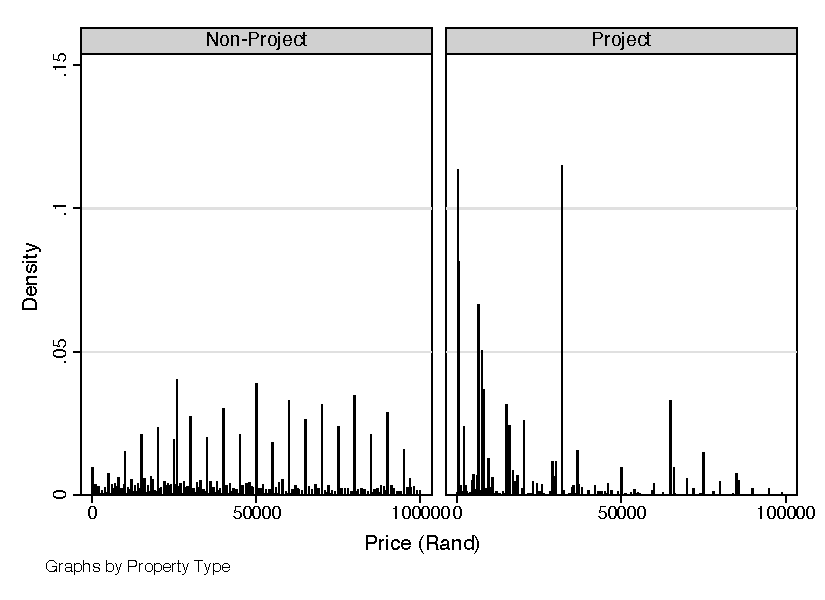
\includegraphics[scale=1]{figures/price_histogram.pdf}\\
Note: Transactions are censored at R100,000.
\end{figure}


\subsubsection{Pre-Existing Formal Dwellings:}  

% pre-existing transactions : 38468 / 127600 = 30\%

We exclude transactions that occur on land plots with at least one preexisting formal residential structure in the 2001 building census (31\% of remaining records).  This method not only helps to reduce error in matching seller identities to housing programs, but also works to distinguish new housing projects from titling, home loan, or other programs that may have been implemented by local housing agencies over the same time period.   

\subsubsection{Spatial Clustering:}  Since housing projects are characterized by large plots of adjacent dwellings, we use a density-based clustering algorithm to group transactions that satisfy the above criteria according to their geographic proximity.  By eliminating loosely clustered or singleton transactions, this method additionally helps to distinguish large housing projects from other small-scale housing programs.  

\begin{figure}
\caption{Convex Hull Example}\label{figure:conhull}
\centering
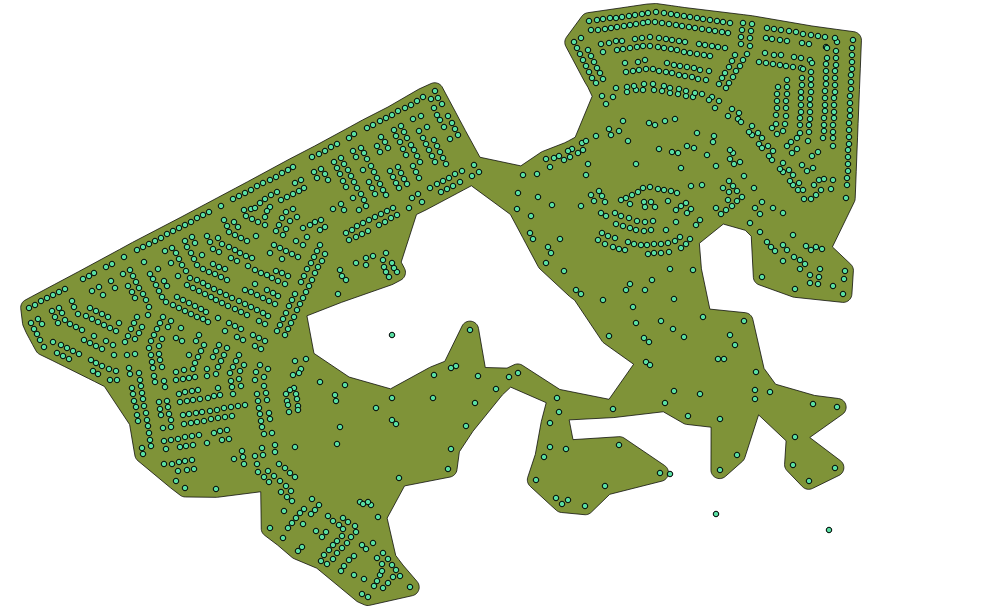
\includegraphics[scale=.27]{figures/rdp_conhull_pic.png}
\end{figure}

\subsubsection{Temporal Clustering:}  Because our empirical design exploits the sudden timing of project construction, we assign a date for each housing project according to the modal year of transactions for houses within each project.  We then include only clusters where over 50\% of transactions occur during the modal year.  This approach rules out incremental projects as well as helps to exclude possible land titling programs, allowing us to leverage the sharp timing of large project construction in our identification.  


%\begin{enumerate}
%	\item \textbf{Seller Identity:}  We focus on transactions from government entities or housing authorities from seller name records.  To %account for large developers or banks being listed as sellers for housing projects, we also include seller names that appear most %frequently.  We exclude transactions flagged as large buildings used for commercial purposes.
%	\item \textbf{Subsidy Value:}  We exclude transactions with purchase prices that are more than R50,000 above the yearly subsidy value.
%	\item \textbf{Pre-Existing Formal Dwellings:}  We exclude transactions that occur on land plots with at least one pre-existing formal %residential structure in the 2001 building census.  This method not only helps to reduce error in matching seller identities to housing %programs, but also works to distinguish new housing projects from titling, home loan, or other programs that may have been implemented %by local housing agencies over the same time period.
%	\item \textbf{Spatial Clustering:}  Since housing projects are characterized by large plots of adjacent dwellings, we use a %density-based clustering algorithm to group transactions that satisfy the above criteria according to their geographic proximity.  By %eliminating loosely clustered or singleton transactions, this method additionally helps to distinguish large housing projects from other %small-scale housing programs.
%	\item \textbf{Temporal Clustering:}  Because our empirical design exploits the sudden timing of project construction, we assign a date %for each housing project according to the modal year of transactions for houses within each project.  We then include only clusters %where over 50\% of transactions occur during the modal year.  This approach rules out gradual construction 
%\end{enumerate}

We validate our measure of housing projects using administrative spatial data from the Gauteng government, which maps a subsample of [XX] housing projects.  Following Figure [XX] (put a nice map here), we find a substantial degree of overlap between our measure and the administrative subsample.  SHOW MAP PLEASE!!!

\subsubsection{Defining Planned but Unconstructed Housing Projects}

The administrative spatial data identifies many project areas that do not appear to have received housing projects, as measured by comparing changes in formal structure counts between the 2001 and 2011 building censuses.  We use these areas to create a sample of planned but unconstructed housing projects to serve as counterfactuals areas in our analysis.

To construct an estimated completion date for planned but unconstructed housing projects, we digitized National Treasury budget reports that detail the start date, expected completion date, and cost of each housing project.  We use a fuzzy-string matching algorithm with bigrams to successfully link project names from the budget reports to over 300 project names in our administrative spatial data (including both completed and uncompleted projects).  We find that for completed projects, the mode transaction year observed in the deeds data falls an average of three years after the start date indicated in the budget reports.  In other words, beneficiaries receive title to their new houses about three years after the housing program is announced in the budget.  Therefore, we assign a expected completion date for unconstructed projects that is three years after the announced start-date in the project.

To differentiate between greenfield and in-situ upgrading projects, we use the building survey to measure the density of informal structures per project area in 2001, prior to the construction of large housing projects.


\begin{table}
	\centering
	\caption{Housing Project Descriptives}\label{table:projectdescriptives}
\begin{tabu}{lcccccc}
 & \multicolumn{2}{c}{Greenfield} & \multicolumn{2}{c}{In-Situ} & \multicolumn{2}{c}{Control} \\ \\[-0.97em] \cline{2-7} 
 & 2001 & 2011 & 2001 & 2011 & 2001 & 2011  \\
\midrule
 Formal Structures  & 456.8  & 1,464.9  & 518.3  & 1,514.3  & 21.3  & 81.7  \\ 
 Informal Structures  & 88.4  & 1,135.8  & 1,624.7  & 1,019.7  & 1,783.5  & 2,477.3  \\ 
 &  &  &  &  &  &  \\ 
 Area (km2)  & \multicolumn{2}{c}{1.17}  & \multicolumn{2}{c}{1.20}  & \multicolumn{2}{c}{2.47}  \\ 
 Total Projects   & \multicolumn{2}{c}{79}  & \multicolumn{2}{c}{64}  & \multicolumn{2}{c}{122}  \\ 
\bottomrule
\end{tabu}

\end{table}

In order to focus on public housing projects as separate from land-titling programs or 


We combine this data with 


%% reference a map of BBLU data ?!

For demographic and economic outcomes, we turn to the census of population for 2001 and 2011 includes information about dwelling type, employment, income, and demographics for each household. 




Table~\ref{table:descriptives} provides descriptive statistics dividing transactions between properties outside and inside a 1.2 kilometer radius of the nearest housing project.  We find that 



  The population census  The smallest level of geography available is census block where 

We are able to identify households within a census block,

We use the smallest level of geography available, which leaves us with 1,00



 General Household Survey







We capture demographic responses to the 

and where administrative data on housing projects.  


\begin{table}
	\centering
	\caption{Descriptive Statistics for Transaction Data}\label{table:descriptives}
	\begin{tabu}{lccc}
\toprule
 & Outside Buffer & Inside Buffer & Housing Project \\
\midrule
 Purchase Price (Rand)  & 184,199.6  & 205,891.3  & 142,748.8  \\ 
\rowfont{\footnotesize} & [386,165.1]  & [249,590.1]  & [447,771.6]  \\ 
 &  &  &  \\ 
 Plot Size (m3)  & 585.2  & 421.7  & 270.4  \\ 
\rowfont{\footnotesize} & [2,040.3]  & [1,225.7]  & [179.2]  \\ 
 &  &  &  \\ 
 Sold At Least Once  & 0.316  & 0.318  & 0.338  \\ 
 Median Purchase Year  & 2006  & 2006  & 2006  \\ 
 Distance to Project (meters) &  & 373.0  & \\
 \rowfont{\footnotesize} &  & [415.9]  & \\
\midrule
 Observations  & 275,296  & 94,172  & 108,809  \\ 
\bottomrule
\end{tabu}
 \\
	\vspace{.2cm}
\footnotesize{Buffers include properties within 1.2 kilometers of a housing project.  These data exclude public housing projects themselves.}
\end{table}







{}
\nocite{*}
\singlespacing
\setlength\bibsep{0pt}
\bibliographystyle{abbrvnat}
\bibliography{ref}




% APPENDIX 
\appendix
\doublespacing

\section*{Appendix}

\begin{table}
	\centering
	\caption{Ten Biggest Sellers}\label{table:biggestsellers}
	\begin{tabu}{lc}
\toprule
 Seller Name & Observations \\
\midrule
City Of Johannesburg Metropolitan Municipality & 29,087  \\
City Of Johannesburg & 27,672  \\
City Of Tshwane Metropolitan Municipality & 24,780  \\
Ekurhuleni Metropolitan Municipality & 21,758  \\
Gauteng Provincial Housing Advisory Board & 13,058  \\
{\bf Total Observations }& {\bf 549,704}  \\
\bottomrule
\end{tabu}

\end{table}



\end{document}